\documentclass[12pt,letterpaper]{article}
\usepackage{graphicx,textcomp}
\usepackage{natbib}
\usepackage{setspace}
\usepackage{fullpage}
\usepackage{color}
\usepackage[reqno]{amsmath}
\usepackage{amsthm}
\usepackage{fancyvrb}
\usepackage{amssymb,enumerate}
\usepackage[all]{xy}
\usepackage{endnotes}
\usepackage{lscape}
\newtheorem{com}{Comment}
\usepackage{float}
\usepackage{hyperref}
\newtheorem{lem} {Lemma}
\newtheorem{prop}{Proposition}
\newtheorem{thm}{Theorem}
\newtheorem{defn}{Definition}
\newtheorem{cor}{Corollary}
\newtheorem{obs}{Observation}
\usepackage[compact]{titlesec}
\usepackage{dcolumn}
\usepackage{tikz}
\usetikzlibrary{arrows}
\usepackage{multirow}
\usepackage{xcolor}
\newcolumntype{.}{D{.}{.}{-1}}
\newcolumntype{d}[1]{D{.}{.}{#1}}
\definecolor{light-gray}{gray}{0.65}
\usepackage{url}
\usepackage{listings}
\usepackage{color}
\usepackage{float}
\usepackage[margin=1in]{geometry}

\definecolor{codegreen}{rgb}{0,0.6,0}
\definecolor{codegray}{rgb}{0.5,0.5,0.5}
\definecolor{codepurple}{rgb}{0.58,0,0.82}
\definecolor{backcolour}{rgb}{0.95,0.95,0.92}

\lstdefinestyle{mystyle}{
	backgroundcolor=\color{backcolour},   
	commentstyle=\color{codegreen},
	keywordstyle=\color{magenta},
	numberstyle=\tiny\color{codegray},
	stringstyle=\color{codepurple},
	basicstyle=\footnotesize,
	breakatwhitespace=false,         
	breaklines=true,                 
	captionpos=b,                    
	keepspaces=true,                 
	numbers=left,                    
	numbersep=5pt,                  
	showspaces=false,                
	showstringspaces=false,
	showtabs=false,                  
	tabsize=2
}
\lstset{style=mystyle}
\newcommand{\Sref}[1]{Section~\ref{#1}}
\newtheorem{hyp}{Hypothesis}

\title{Do the stances of Christian churches influence identifiers' politcial beliefs? }
\date{April 3, 2026}
\author{Caroline Kajkowski}


\begin{document}
	\maketitle
\section{Original Study}
\begin{description}
	\item The study I chose to replicate for this project: “The Influence of Religious–Political Sophistication on U.S. Public Opinion” by Eric Schmidt (2017). The main purpose of this study is to discover whether and how religious institutes’ viewpoints affect parishioners' understanding and reasoning on political issues. This phenomenon is referred to as Religious-Political Sophistication (RPS). 
	Other literature on this topic, discuss the direct influence of religious leaders and how these teachings potentially influence religious identifiers' political beliefs/allignment. Schmidt suggests on top of direct influence, religious identifiers also take in account their church's stance on issues (i.e. the Roman Catholic Church's stance on abortion). 
	Therefore, the author is looking to test three hypotheses regarding RPS: 
	\begin{itemize}
		\item Religious identifiers who know their church’s teachings are more likely to share these views
		\item RPS has a greater impact on their public opinion in comparison to secular knowledge
		\item RPS helps connect religious identifers' faith to politics
	\end{itemize}
	\item[Method]
	\item To test the hypotheses above, the author took data from 2014 Cooperative Congressional Election Study (CCES) and an original CCES module. From there, he took the best represented religious traditions (Roman Catholic, Evangelical Protestants, and Mainline Protestants) to analyze their political positions on same sex marriage and abortion. 
\end{description}
\newpage
\section{Data}
	\lstinputlisting[language=R, firstline=14, lastline=19]{rep_models.R} 
	\begin{description}
		\item In the original R script, the author decides to separate the dataset to create two new datasets with all inputs of Roman Catholic and Evangelical Protestants in one and Mainline Protestants in another. The justification for this in the paper was that the author found that the Roman Catholic church and Evangelical Protestants have more clear universal opinions on same sex marriage and abortion rights, while Mainline Protestants have varrying views on these social policies. Therefore, the study is focused on the effect of RPS on Roman Catholic and Evangelical Protestants while treating Mainline Protestants as the baseline to compare later on. 
		\item [Input variables:]
		\item Party ID (0 = strong Democrat; 6 = strong Republican)
		\item Church attendance (0 = never; 5 = more than once per week)
		\item Biblical Literacy (the number of correct answers to three multiple-choice questions about the Bible’s books and figures)
		\item Secular Political Knowledge (a three-point scale indicating each respondent’s number of correct responses to two questions about national politics)
		\item RPS (1 =respondent knows official denomination stance; 0 = respondent doesn't know)
		\item Controled variables: age, ideology, gender, race, education, family income, and religious tradition (1 = Roman Catholic; 0 = Evangelical Protestant) 
		\item[Outcome variable:] 
		\item Support (1 = support rights (same-sex marriage or abortion); 0 = oppose)
	\end{description}
\section{Original Models}
\begin{description}
	\item The author creates binomial logistic regression models that are used throughout the paper:
	\item[Secular Model:]
\begin{align*}
	\text{Support} =\;& \beta_0 
	+ \beta_1 \, \text{Party Identification} 
	+ \beta_2 \, \text{Secular Political Knowledge} \\
	& + \beta_3 \, (\text{Party Identification} \times \text{Secular Political Knowledge}) 
\end{align*}
\item[Naive Model:]
\begin{align*}
	\text{Support} =\;& \beta_0 
	+ \beta_1 \, \text{Party Identification} 
	+ \beta_2 \, \text{Secular Political Knowledge} \\
	& + \beta_3 \, (\text{Party Identification} \times \text{Secular Political Knowledge}) \\
	& + \beta_4 \, \text{Church Attendance} 
	+ \beta_5 \, \text{Biblical Literacy} \\
	& + \beta_6 \, (\text{Church Attendance} \times \text{Biblical Literacy}) 
\end{align*}
\item["Culture Wars" Model:]
\begin{align*}
	\text{Support} =\;& \beta_0 
	+ \beta_1 \, \text{Party Identification} 
	+ \beta_2 \, \text{Secular Political Knowledge} \\
	& + \beta_3 \, (\text{Party Identification} \times \text{Secular Political Knowledge}) \\
	& + \beta_4 \, \text{Church Attendance} 
	+ \beta_5 \, \text{Biblical Literacy} \\
	& + \beta_6 \, (\text{Church Attendance} \times \text{Biblical Literacy}) \\
	& + \beta_7 \, (\text{Church Attendance} \times \text{Secular Political Knowledge}) 
\end{align*}
\item[RPS Model:]
\begin{align*}
	\text{Support} =\;& \beta_0 
	+ \beta_1 \, \text{Party Identification} 
	+ \beta_2 \, \text{Secular Political Knowledge} \\
	& + \beta_3 \, (\text{Party Identification} \times \text{Secular Political Knowledge}) \\
	& + \beta_4 \, \text{Church Attendance} 
	+ \beta_5 \, \text{Biblical Literacy} \\
	& + \beta_6 \, (\text{Church Attendance} \times \text{Biblical Literacy}) \\
	& + \beta_7 \, (\text{Church Attendance} \times \text{Secular Political Knowledge}) \\
	& + \beta_8 \, \text{RPS} \\
	& + \beta_9 \, (\text{Church Attendance} \times \text{RPS}) 
\end{align*}
\item Tables 1 and 2 in this paper look at Evangelical Protestants and Roman Catholics support of same-sex marriage and abortion rights (respectively) using all four models above. The author concludes that the secular models provides insight 
\item Table 3 takes a different approach and looks at whether the respondent's stance on same sex marriage predicts their stance on abortion. So the model looks a bit different (shown in the code below) 
\lstinputlisting[language=R, firstline=104, lastline=119]{rep_models.R} 
\item Tables 4 and 5 look at the Mainline Protestants. As mentioned before, the data was split into two datasets because the author believed that Mainline protestants have more mixed views on this topics in comparison to Roman Catholics and Evangelical Protestants. The author also chose to not include all the demographic variables in the Mainline Protestant models. 
\item Tables 6 and 7 
\lstinputlisting[language=R, firstline=192, lastline=238]{rep_models.R} 
\item Table 8
\lstinputlisting[language=R, firstline=242, lastline=258]{rep_models.R} 
\end{description}
\begin{table}[!htbp] \centering 
	\caption{Evangelical Protestants and Roman Catholics' support of SSM Replication} 
	\label{} 
	\scriptsize 
	\begin{tabular}{@{\extracolsep{5pt}}lcccc} 
		\\[-1.8ex]\hline 
		\hline \\[-1.8ex] 
		& \multicolumn{4}{c}{\textit{Dependent variable:}} \\ 
		\cline{2-5} 
		\\[-1.8ex] & \multicolumn{4}{c}{ssm} \\ 
		& Secular & Naive & Culture Wars & RPS \\ 
		\\[-1.8ex] & (1) & (2) & (3) & (4)\\ 
		\hline \\[-1.8ex] 
		age & $-$0.025$^{**}$ & $-$0.025$^{**}$ & $-$0.025$^{**}$ & $-$0.032$^{**}$ \\ 
		& (0.011) & (0.013) & (0.013) & (0.015) \\ 
		& & & & \\ 
		female & 0.533$^{*}$ & 0.481 & 0.478 & 0.726$^{*}$ \\ 
		& (0.323) & (0.351) & (0.352) & (0.400) \\ 
		& & & & \\ 
		black & 0.059 & $-$0.138 & $-$0.140 & $-$0.331 \\ 
		& (0.493) & (0.586) & (0.586) & (0.633) \\ 
		& & & & \\ 
		education.collapsed & 0.055 & 0.075 & 0.076 & 0.014 \\ 
		& (0.126) & (0.144) & (0.144) & (0.165) \\ 
		& & & & \\ 
		income.collapsed & 0.013 & 0.037 & 0.038 & 0.048 \\ 
		& (0.058) & (0.063) & (0.064) & (0.072) \\ 
		& & & & \\ 
		ideology.collapsed & $-$0.830$^{***}$ & $-$0.793$^{***}$ & $-$0.795$^{***}$ & $-$0.922$^{***}$ \\ 
		& (0.250) & (0.281) & (0.281) & (0.313) \\ 
		& & & & \\ 
		romancatholic & 1.571$^{***}$ & 1.303$^{***}$ & 1.309$^{***}$ & 1.111$^{***}$ \\ 
		& (0.336) & (0.366) & (0.371) & (0.409) \\ 
		& & & & \\ 
		partyid & $-$0.249$^{*}$ & $-$0.242 & $-$0.245 & $-$0.183 \\ 
		& (0.143) & (0.163) & (0.165) & (0.197) \\ 
		& & & & \\ 
		secular.knowledge & $-$0.082 & $-$0.141 & $-$0.108 & 0.040 \\ 
		& (0.308) & (0.354) & (0.471) & (0.519) \\ 
		& & & & \\ 
		church &  & $-$0.080 & $-$0.061 & 0.044 \\ 
		&  & (0.263) & (0.322) & (0.378) \\ 
		& & & & \\ 
		bible.collapsed &  & $-$0.262 & $-$0.261 & $-$0.084 \\ 
		&  & (0.512) & (0.511) & (0.550) \\ 
		& & & & \\ 
		rps.ssm &  &  &  & $-$0.596 \\ 
		&  &  &  & (0.764) \\ 
		& & & & \\ 
		partyid:secular.knowledge & $-$0.002 & 0.002 & 0.004 & $-$0.078 \\ 
		& (0.088) & (0.098) & (0.099) & (0.116) \\ 
		& & & & \\ 
		church:bible.collapsed &  & $-$0.074 & $-$0.074 & $-$0.054 \\ 
		&  & (0.171) & (0.170) & (0.185) \\ 
		& & & & \\ 
		secular.knowledge:church &  &  & $-$0.014 & 0.075 \\ 
		&  &  & (0.138) & (0.159) \\ 
		& & & & \\ 
		church:rps.ssm &  &  &  & $-$0.605$^{**}$ \\ 
		&  &  &  & (0.262) \\ 
		& & & & \\ 
		Constant & 1.848$^{**}$ & 2.848$^{**}$ & 2.800$^{**}$ & 3.446$^{**}$ \\ 
		& (0.834) & (1.148) & (1.236) & (1.384) \\ 
		& & & & \\ 
		\hline \\[-1.8ex] 
		Observations & 280 & 246 & 246 & 246 \\ 
		Log Likelihood & $-$139.734 & $-$118.555 & $-$118.549 & $-$97.484 \\ 
		Akaike Inf. Crit. & 301.468 & 265.110 & 267.099 & 228.969 \\ 
		\hline 
		\hline \\[-1.8ex] 
		\textit{Note:}  & \multicolumn{4}{r}{$^{*}$p$<$0.1; $^{**}$p$<$0.05; $^{***}$p$<$0.01} \\ 
	\end{tabular} 
\end{table} 
\begin{table}[!htbp] \centering 
	\caption{Evangelical Protestants and Roman Catholics' support of abortion Replication} 
	\label{} 
	\scriptsize 
	\begin{tabular}{@{\extracolsep{5pt}}lcccc} 
		\\[-1.8ex]\hline 
		\hline \\[-1.8ex] 
		& \multicolumn{4}{c}{\textit{Dependent variable:}} \\ 
		\cline{2-5} 
		\\[-1.8ex] & \multicolumn{4}{c}{abortion} \\ 
		& Secular & Naive & Culture Wars & RPS \\ 
		\\[-1.8ex] & (1) & (2) & (3) & (4)\\ 
		\hline \\[-1.8ex] 
		age & $-$0.012 & $-$0.019 & $-$0.019 & $-$0.019 \\ 
		& (0.011) & (0.013) & (0.013) & (0.013) \\ 
		& & & & \\ 
		female & 0.419 & 0.298 & 0.297 & 0.319 \\ 
		& (0.326) & (0.363) & (0.364) & (0.371) \\ 
		& & & & \\ 
		black & 0.411 & $-$0.085 & $-$0.087 & $-$0.150 \\ 
		& (0.505) & (0.629) & (0.631) & (0.629) \\ 
		& & & & \\ 
		education.collapsed & $-$0.069 & $-$0.042 & $-$0.042 & $-$0.067 \\ 
		& (0.128) & (0.150) & (0.151) & (0.155) \\ 
		& & & & \\ 
		income.collapsed & 0.077 & 0.036 & 0.036 & 0.036 \\ 
		& (0.059) & (0.065) & (0.065) & (0.067) \\ 
		& & & & \\ 
		ideology.collapsed & $-$1.120$^{***}$ & $-$1.320$^{***}$ & $-$1.320$^{***}$ & $-$1.361$^{***}$ \\ 
		& (0.255) & (0.310) & (0.310) & (0.315) \\ 
		& & & & \\ 
		romancatholic & 0.921$^{***}$ & 0.775$^{**}$ & 0.776$^{**}$ & 0.657$^{*}$ \\ 
		& (0.328) & (0.371) & (0.377) & (0.385) \\ 
		& & & & \\ 
		partyid & $-$0.171 & $-$0.150 & $-$0.151 & $-$0.127 \\ 
		& (0.140) & (0.163) & (0.168) & (0.174) \\ 
		& & & & \\ 
		secular.knowledge & $-$0.124 & $-$0.250 & $-$0.242 & $-$0.252 \\ 
		& (0.314) & (0.366) & (0.473) & (0.477) \\ 
		& & & & \\ 
		church &  & 0.565$^{**}$ & 0.569$^{*}$ & 0.661$^{*}$ \\ 
		&  & (0.271) & (0.326) & (0.349) \\ 
		& & & & \\ 
		bible.collapsed &  & 1.105$^{**}$ & 1.104$^{**}$ & 1.095$^{**}$ \\ 
		&  & (0.511) & (0.512) & (0.517) \\ 
		& & & & \\ 
		rps.ssm &  &  &  & 0.162 \\ 
		&  &  &  & (0.732) \\ 
		& & & & \\ 
		partyid:secular.knowledge & $-$0.059 & $-$0.056 & $-$0.055 & $-$0.069 \\ 
		& (0.088) & (0.100) & (0.102) & (0.105) \\ 
		& & & & \\ 
		church:bible.collapsed &  & $-$0.530$^{***}$ & $-$0.530$^{***}$ & $-$0.493$^{***}$ \\ 
		&  & (0.179) & (0.179) & (0.179) \\ 
		& & & & \\ 
		secular.knowledge:church &  &  & $-$0.004 & 0.020 \\ 
		&  &  & (0.142) & (0.146) \\ 
		& & & & \\ 
		church:rps.ssm &  &  &  & $-$0.324 \\ 
		&  &  &  & (0.241) \\ 
		& & & & \\ 
		Constant & 1.898$^{**}$ & 2.085$^{*}$ & 2.074$^{*}$ & 2.090$^{*}$ \\ 
		& (0.839) & (1.095) & (1.174) & (1.202) \\ 
		& & & & \\ 
		\hline \\[-1.8ex] 
		Observations & 279 & 245 & 245 & 245 \\ 
		Log Likelihood & $-$138.275 & $-$112.479 & $-$112.478 & $-$109.516 \\ 
		Akaike Inf. Crit. & 298.551 & 252.957 & 254.957 & 253.033 \\ 
		\hline 
		\hline \\[-1.8ex] 
		\textit{Note:}  & \multicolumn{4}{r}{$^{*}$p$<$0.1; $^{**}$p$<$0.05; $^{***}$p$<$0.01} \\ 
	\end{tabular} 
\end{table} 
\begin{table}[!htbp] \centering 
	\caption{RPS does not promote cross-over issue constraint for Evangelical Protestants and Roman Catholics} 
	\label{} 
	\scriptsize 
	\begin{tabular}{@{\extracolsep{5pt}}lcc} 
		\\[-1.8ex]\hline 
		\hline \\[-1.8ex] 
		& \multicolumn{2}{c}{\textit{}} \\ 
		\cline{2-3} 
		\\[-1.8ex] \\ 
		& SSM Support & Abortion Support \\ 
		\\[-1.8ex] & (1) & (2)\\ 
		\hline \\[-1.8ex] 
		age & $-$0.023$^{*}$ & $-$0.019 \\ 
		& (0.013) & (0.013) \\ 
		& & \\ 
		female & 0.549 & 0.319 \\ 
		& (0.370) & (0.371) \\ 
		& & \\ 
		black & $-$0.537 & $-$0.150 \\ 
		& (0.605) & (0.629) \\ 
		& & \\ 
		education.collapsed & 0.125 & $-$0.067 \\ 
		& (0.155) & (0.155) \\ 
		& & \\ 
		income.collapsed & 0.041 & 0.036 \\ 
		& (0.067) & (0.067) \\ 
		& & \\ 
		ideology.collapsed & $-$0.868$^{***}$ & $-$1.361$^{***}$ \\ 
		& (0.290) & (0.315) \\ 
		& & \\ 
		romancatholic & 1.128$^{***}$ & 0.657$^{*}$ \\ 
		& (0.390) & (0.385) \\ 
		& & \\ 
		partyid & $-$0.179 & $-$0.127 \\ 
		& (0.169) & (0.174) \\ 
		& & \\ 
		secular.knowledge & $-$0.036 & $-$0.252 \\ 
		& (0.493) & (0.477) \\ 
		& & \\ 
		church & 0.013 & 0.661$^{*}$ \\ 
		& (0.336) & (0.349) \\ 
		& & \\ 
		bible.collapsed & $-$0.411 & 1.095$^{**}$ \\ 
		& (0.526) & (0.517) \\ 
		& & \\ 
		rps.abortion & 0.003 &  \\ 
		& (0.758) &  \\ 
		& & \\ 
		rps.ssm &  & 0.162 \\ 
		&  & (0.732) \\ 
		& & \\ 
		partyid:secular.knowledge & $-$0.037 & $-$0.069 \\ 
		& (0.102) & (0.105) \\ 
		& & \\ 
		church:bible.collapsed & 0.039 & $-$0.493$^{***}$ \\ 
		& (0.182) & (0.179) \\ 
		& & \\ 
		secular.knowledge:church & 0.014 & 0.020 \\ 
		& (0.145) & (0.146) \\ 
		& & \\ 
		church:rps.abortion & $-$0.411 &  \\ 
		& (0.251) &  \\ 
		& & \\ 
		church:rps.ssm &  & $-$0.324 \\ 
		&  & (0.241) \\ 
		& & \\ 
		Constant & 2.746$^{**}$ & 2.090$^{*}$ \\ 
		& (1.272) & (1.202) \\ 
		& & \\ 
		\hline \\[-1.8ex] 
		Observations & 246 & 245 \\ 
		Log Likelihood & $-$112.603 & $-$109.516 \\ 
		Akaike Inf. Crit. & 259.206 & 253.033 \\ 
		\hline 
		\hline \\[-1.8ex] 
		\textit{Note:}  & \multicolumn{2}{r}{$^{*}$p$<$0.1; $^{**}$p$<$0.05; $^{***}$p$<$0.01} \\ 
	\end{tabular} 
\end{table} 
\begin{table}[!htbp] \centering 
	\caption{Mainline Protestants' support of SSM Replication} 
	\label{} 
	\scriptsize 
	\begin{tabular}{@{\extracolsep{5pt}}lcccc} 
		\\[-1.8ex]\hline 
		\hline \\[-1.8ex] 
		& \multicolumn{4}{c}{\textit{Dependent variable:}} \\ 
		\cline{2-5} 
		\\[-1.8ex] & \multicolumn{4}{c}{ssm} \\ 
		& Secular & Naive & Culture Wars & RPS \\ 
		\\[-1.8ex] & (1) & (2) & (3) & (4)\\ 
		\hline \\[-1.8ex] 
		partyid & $-$0.182 & $-$0.095 & $-$0.080 & $-$0.064 \\ 
		& (0.165) & (0.178) & (0.181) & (0.188) \\ 
		& & & & \\ 
		secular.knowledge & 0.911$^{*}$ & 0.924$^{*}$ & 0.646 & 0.579 \\ 
		& (0.499) & (0.508) & (0.696) & (0.718) \\ 
		& & & & \\ 
		church &  & $-$0.365 & $-$0.436 & $-$0.455 \\ 
		&  & (0.439) & (0.459) & (0.482) \\ 
		& & & & \\ 
		bible.collapsed &  & $-$0.130 & 0.010 & $-$0.113 \\ 
		&  & (0.652) & (0.703) & (0.716) \\ 
		& & & & \\ 
		rps.ssm &  &  &  & 0.633 \\ 
		&  &  &  & (1.063) \\ 
		& & & & \\ 
		partyid:secular.knowledge & $-$0.176 & $-$0.229$^{*}$ & $-$0.236$^{*}$ & $-$0.241$^{*}$ \\ 
		& (0.120) & (0.127) & (0.128) & (0.130) \\ 
		& & & & \\ 
		church:bible.collapsed &  & 0.140 & 0.083 & 0.108 \\ 
		&  & (0.275) & (0.294) & (0.301) \\ 
		& & & & \\ 
		secular.knowledge:church &  &  & 0.131 & 0.120 \\ 
		&  &  & (0.226) & (0.238) \\ 
		& & & & \\ 
		church:rps.ssm &  &  &  & 0.058 \\ 
		&  &  &  & (0.416) \\ 
		& & & & \\ 
		Constant & 0.509 & 0.905 & 1.000 & 0.715 \\ 
		& (0.624) & (1.103) & (1.125) & (1.153) \\ 
		& & & & \\ 
		\hline \\[-1.8ex] 
		Observations & 91 & 82 & 82 & 82 \\ 
		Log Likelihood & $-$52.919 & $-$47.535 & $-$47.366 & $-$46.415 \\ 
		Akaike Inf. Crit. & 113.837 & 109.070 & 110.731 & 112.829 \\ 
		\hline 
		\hline \\[-1.8ex] 
		\textit{Note:}  & \multicolumn{4}{r}{$^{*}$p$<$0.1; $^{**}$p$<$0.05; $^{***}$p$<$0.01} \\ 
	\end{tabular} 
\end{table} 
\begin{table}[!htbp] \centering 
	\caption{Mainline Protestants' support of Abortion Replication} 
	\label{} 
	\scriptsize 
	\begin{tabular}{@{\extracolsep{5pt}}lcccc} 
		\\[-1.8ex]\hline 
		\hline \\[-1.8ex] 
		& \multicolumn{4}{c}{\textit{Dependent variable:}} \\ 
		\cline{2-5} 
		\\[-1.8ex] & \multicolumn{4}{c}{abortion} \\ 
		& Secular & Naive & Culture Wars & RPS \\ 
		\\[-1.8ex] & (1) & (2) & (3) & (4)\\ 
		\hline \\[-1.8ex] 
		partyid & $-$0.309$^{*}$ & $-$0.290 & $-$0.233 & $-$0.239 \\ 
		& (0.174) & (0.191) & (0.200) & (0.203) \\ 
		& & & & \\ 
		secular.knowledge & 0.557 & 0.503 & $-$0.754 & $-$0.714 \\ 
		& (0.537) & (0.559) & (0.801) & (0.819) \\ 
		& & & & \\ 
		church &  & $-$0.214 & $-$0.607 & $-$0.606 \\ 
		&  & (0.438) & (0.492) & (0.504) \\ 
		& & & & \\ 
		bible.collapsed &  & 0.025 & 0.814 & 0.850 \\ 
		&  & (0.679) & (0.842) & (0.856) \\ 
		& & & & \\ 
		rps.ssm &  &  &  & $-$0.183 \\ 
		&  &  &  & (1.186) \\ 
		& & & & \\ 
		partyid:secular.knowledge & $-$0.123 & $-$0.153 & $-$0.221 & $-$0.226 \\ 
		& (0.125) & (0.134) & (0.146) & (0.147) \\ 
		& & & & \\ 
		church:bible.collapsed &  & 0.169 & $-$0.106 & $-$0.109 \\ 
		&  & (0.281) & (0.325) & (0.329) \\ 
		& & & & \\ 
		secular.knowledge:church &  &  & 0.632$^{**}$ & 0.635$^{**}$ \\ 
		&  &  & (0.262) & (0.266) \\ 
		& & & & \\ 
		church:rps.ssm &  &  &  & $-$0.036 \\ 
		&  &  &  & (0.437) \\ 
		& & & & \\ 
		Constant & 1.338$^{*}$ & 1.329 & 1.868 & 1.970 \\ 
		& (0.697) & (1.164) & (1.284) & (1.341) \\ 
		& & & & \\ 
		\hline \\[-1.8ex] 
		Observations & 93 & 84 & 84 & 84 \\ 
		Log Likelihood & $-$51.172 & $-$44.908 & $-$41.624 & $-$41.520 \\ 
		Akaike Inf. Crit. & 110.345 & 103.817 & 99.248 & 103.039 \\ 
		\hline 
		\hline \\[-1.8ex] 
		\textit{Note:}  & \multicolumn{4}{r}{$^{*}$p$<$0.1; $^{**}$p$<$0.05; $^{***}$p$<$0.01} \\ 
	\end{tabular} 
\end{table} 
\begin{table}[!htbp] \centering 
	\caption{Beliefs about church teaching on same-sex marriage by personal opinion on same-sex marriage Replication} 
	\label{} 
	\begin{tabular}{@{\extracolsep{5pt}} ccc} 
		\\[-1.8ex]\hline 
		\hline \\[-1.8ex] 
		& Opposes & Supports \\ 
		\hline \\[-1.8ex] 
		Church supports SSM & $0.04$ & $0.50$ \\ 
		Church supports civil unions & $0.25$ & $0.15$ \\ 
		Church opposes SSM & $0.62$ & $0.15$ \\ 
		Doesn't know & $0.10$ & $0.20$ \\ 
		Total & $1.00$ & $1.00$ \\ 
		n & $199$ & $201$ \\ 
		\hline \\[-1.8ex] 
	\end{tabular} 
\end{table} 
\begin{table}[!htbp] \centering 
	\caption{Beliefs about church teaching on abortion by personal opinion on unrestricted abortion rights Replication} 
	\label{} 
	\begin{tabular}{@{\extracolsep{5pt}} cccc} 
		\\[-1.8ex]\hline 
		\hline \\[-1.8ex] 
		& 0 & 1 & NA \\ 
		\hline \\[-1.8ex] 
		1 & Always Permit & 0 & $0.01$ \\ 
		2 & DK & 0 & $0.06$ \\ 
		3 & Establish Need & 0 & $0.08$ \\ 
		4 & Never Permit & 0 & $0.39$ \\ 
		5 & Standard GOP Exceptions & 0 & $0.45$ \\ 
		6 & Always Permit & 1 & $0.34$ \\ 
		7 & DK & 1 & $0.16$ \\ 
		8 & Establish Need & 1 & $0.14$ \\ 
		9 & Never Permit & 1 & $0.17$ \\ 
		10 & Standard GOP Exceptions & 1 & $0.19$ \\ 
		\hline \\[-1.8ex] 
	\end{tabular} 
\end{table} 
\begin{table}[!htbp] \centering 
	\caption{Incorrect RPS reports only influence political attitudes through church attendance: support for same-sex marriage and unrestricted abortion rights, evangelical Protestants and Roman Catholics Replication} 
	\label{} 
	\scriptsize 
	\begin{tabular}{@{\extracolsep{5pt}}lcc} 
		\\[-1.8ex]\hline 
		\hline \\[-1.8ex] 
		& \multicolumn{2}{c}{\textit{Dependent variable:}} \\ 
		\cline{2-3} 
		\\[-1.8ex] & ssm & abortion \\ 
		& SSM Support & Abortion Support \\ 
		\\[-1.8ex] & (1) & (2)\\ 
		\hline \\[-1.8ex] 
		age & $-$0.029$^{**}$ & $-$0.014 \\ 
		& (0.014) & (0.014) \\ 
		& & \\ 
		female & 0.686$^{*}$ & 0.390 \\ 
		& (0.378) & (0.386) \\ 
		& & \\ 
		black & $-$0.287 & $-$0.705 \\ 
		& (0.614) & (0.678) \\ 
		& & \\ 
		education.collapsed & 0.048 & 0.008 \\ 
		& (0.155) & (0.168) \\ 
		& & \\ 
		income.collapsed & 0.049 & 0.050 \\ 
		& (0.068) & (0.069) \\ 
		& & \\ 
		ideology.collapsed & $-$0.917$^{***}$ & $-$1.397$^{***}$ \\ 
		& (0.304) & (0.324) \\ 
		& & \\ 
		romancatholic & 1.127$^{***}$ & 0.493 \\ 
		& (0.393) & (0.423) \\ 
		& & \\ 
		partyid & $-$0.236 & $-$0.127 \\ 
		& (0.181) & (0.180) \\ 
		& & \\ 
		secular.knowledge & $-$0.095 & $-$0.202 \\ 
		& (0.500) & (0.489) \\ 
		& & \\ 
		church & $-$0.096 & 0.309 \\ 
		& (0.338) & (0.361) \\ 
		& & \\ 
		bible.collapsed & $-$0.123 & 1.028$^{*}$ \\ 
		& (0.527) & (0.530) \\ 
		& & \\ 
		incorrect.rps.ssm & 0.275 &  \\ 
		& (0.750) &  \\ 
		& & \\ 
		incorrect.rps.abortion &  & $-$0.734 \\ 
		&  & (0.828) \\ 
		& & \\ 
		partyid:secular.knowledge & $-$0.012 & $-$0.088 \\ 
		& (0.108) & (0.108) \\ 
		& & \\ 
		church:bible.collapsed & $-$0.148 & $-$0.472$^{**}$ \\ 
		& (0.178) & (0.189) \\ 
		& & \\ 
		secular.knowledge:church & $-$0.033 & $-$0.039 \\ 
		& (0.148) & (0.156) \\ 
		& & \\ 
		church:incorrect.rps.ssm & 0.492$^{*}$ &  \\ 
		& (0.251) &  \\ 
		& & \\ 
		church:incorrect.rps.abortion &  & 0.790$^{***}$ \\ 
		&  & (0.287) \\ 
		& & \\ 
		Constant & 2.831$^{**}$ & 2.192 \\ 
		& (1.343) & (1.342) \\ 
		& & \\ 
		\hline \\[-1.8ex] 
		Observations & 246 & 245 \\ 
		Log Likelihood & $-$106.152 & $-$102.855 \\ 
		Akaike Inf. Crit. & 246.303 & 239.709 \\ 
		\hline 
		\hline \\[-1.8ex] 
		\textit{Note:}  & \multicolumn{2}{r}{$^{*}$p$<$0.1; $^{**}$p$<$0.05; $^{***}$p$<$0.01} \\ 
	\end{tabular} 
\end{table} 
\clearpage
\section{Original Figures}
\begin{figure}[H]
	\centering
	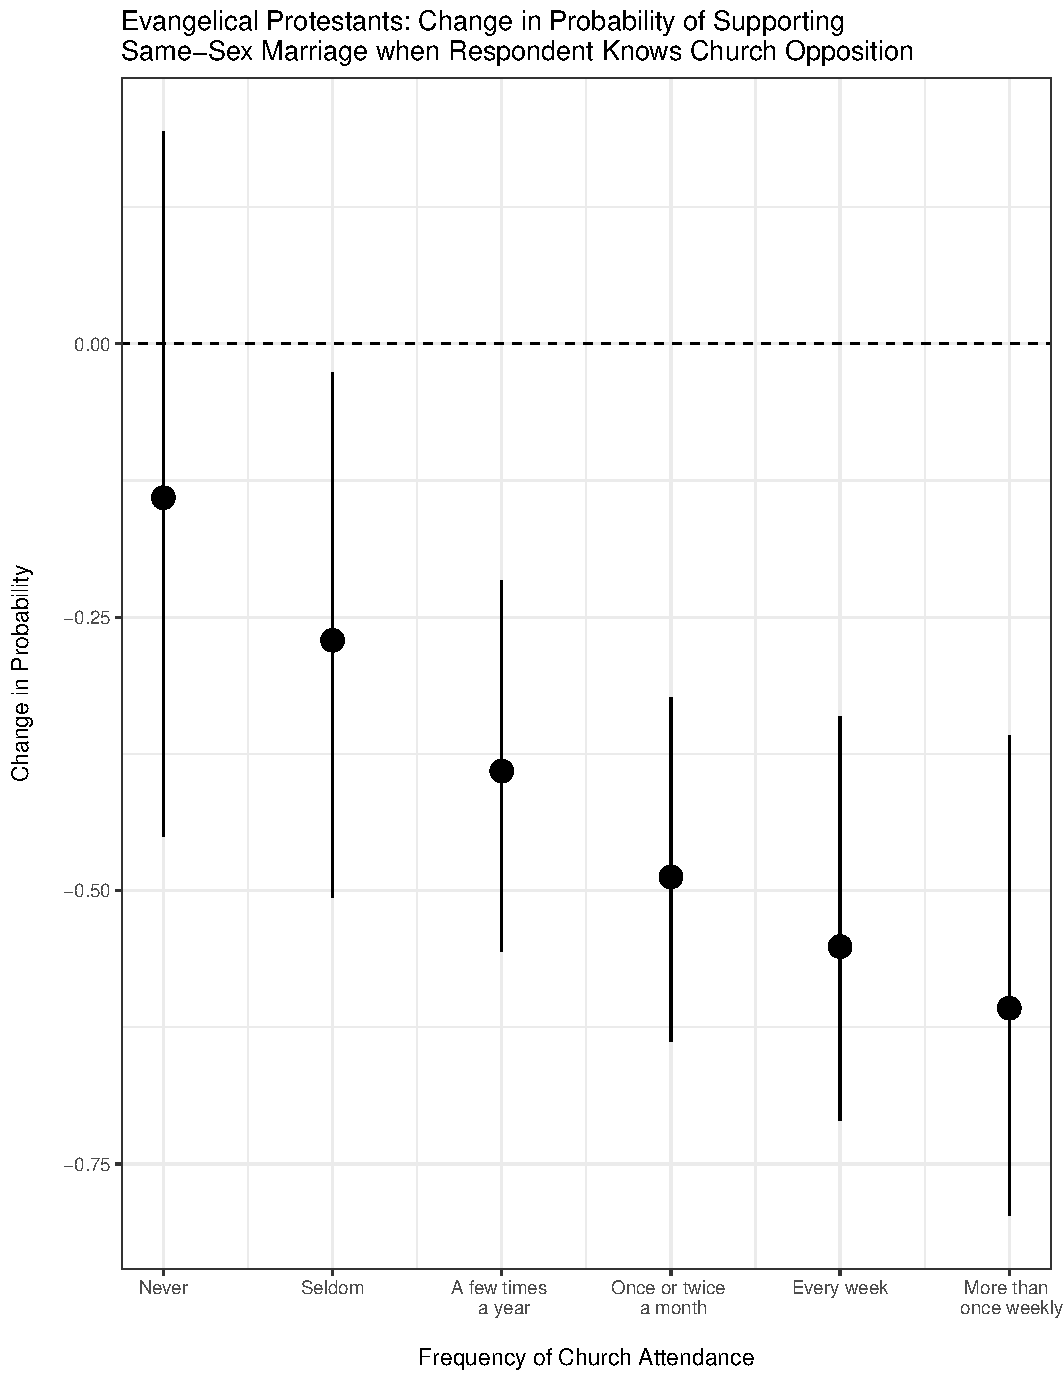
\includegraphics[width=0.45\textwidth]{Fig1.pdf}
	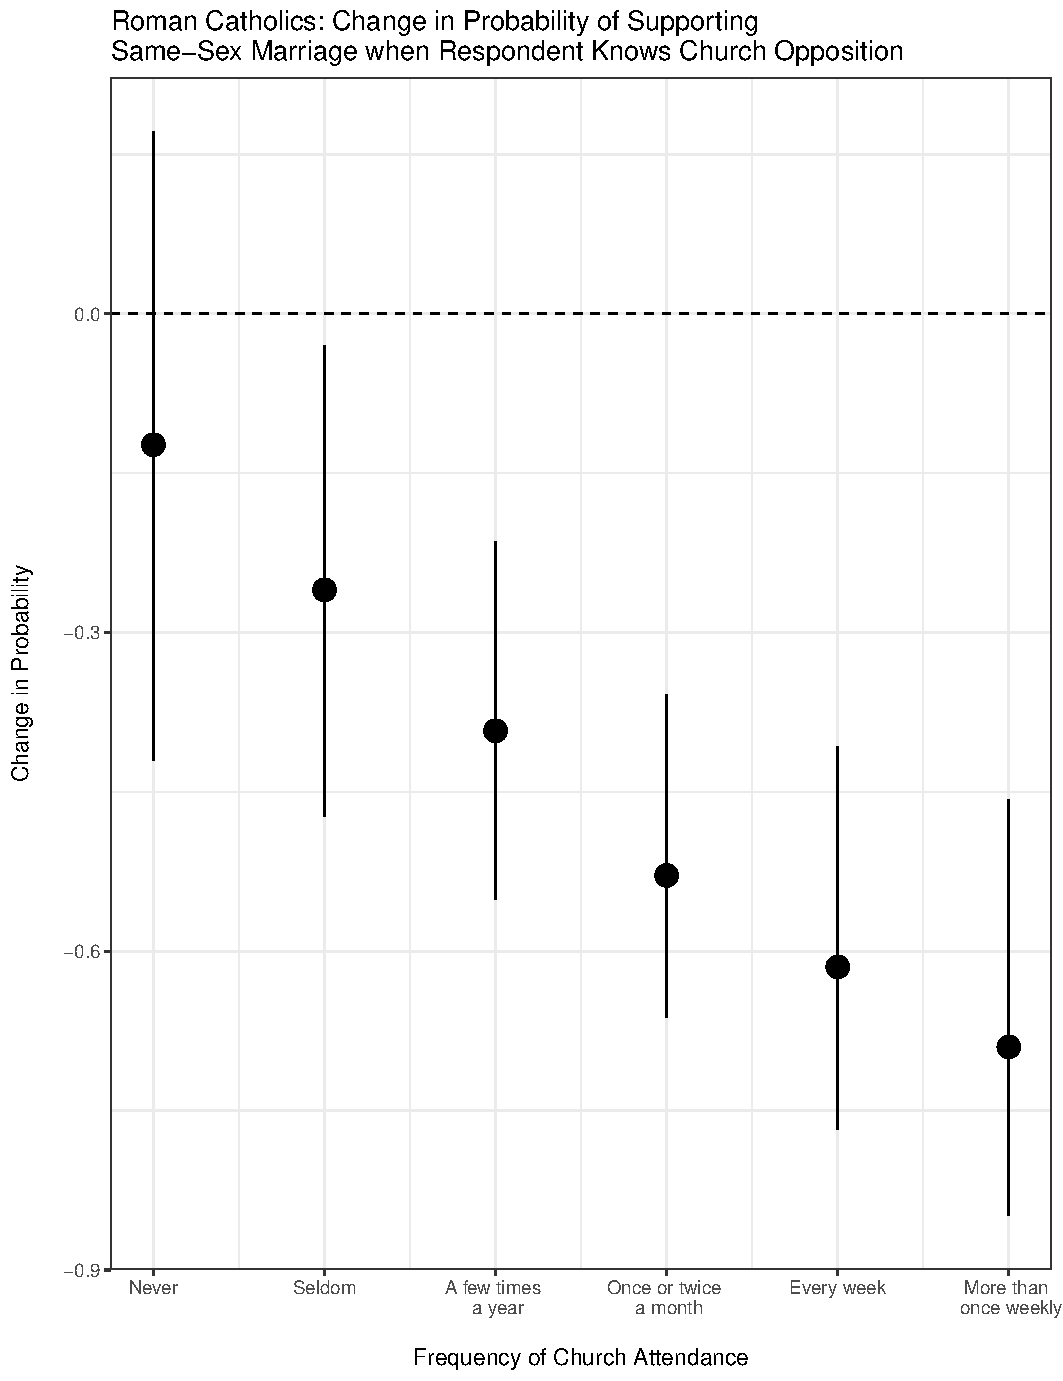
\includegraphics[width=0.45\textwidth]{Fig2.pdf} \\
	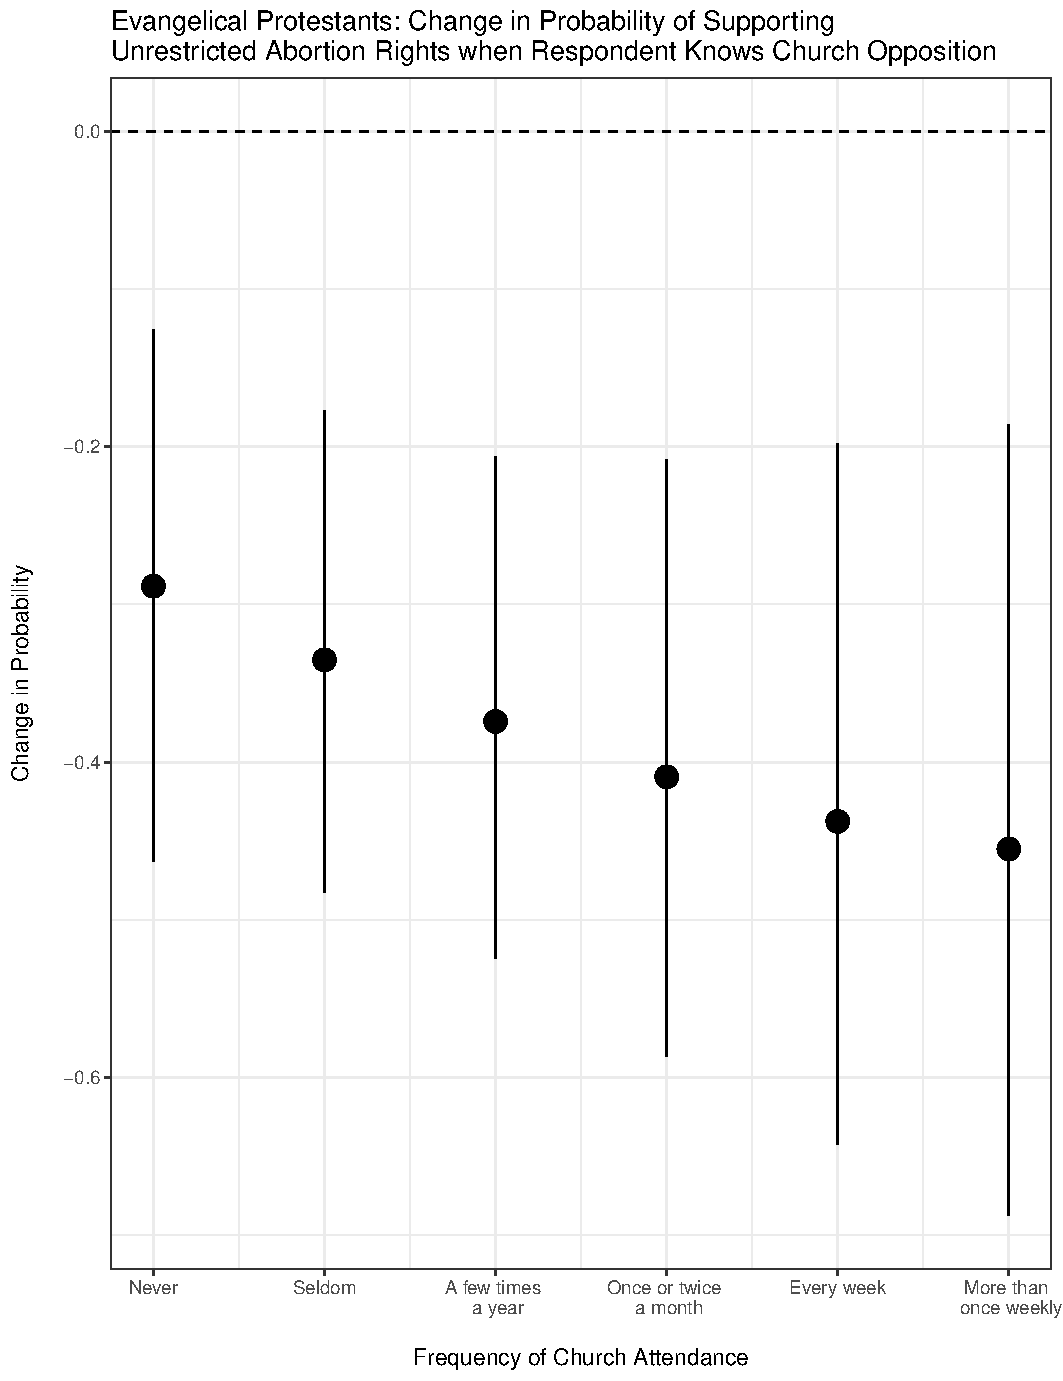
\includegraphics[width=0.45\textwidth]{Fig3.pdf}
	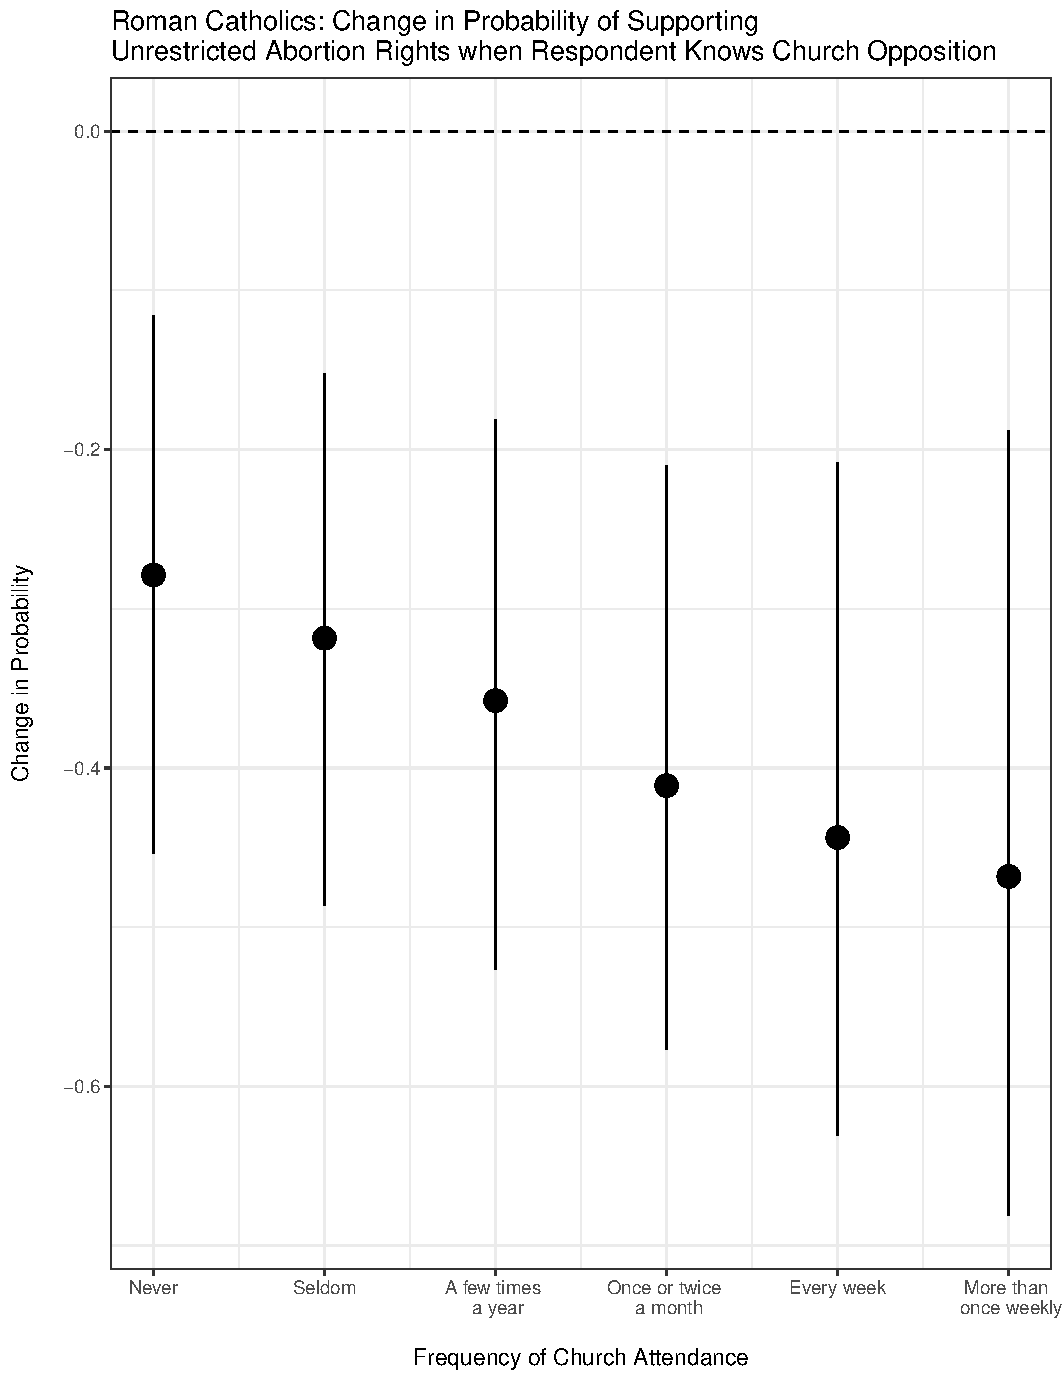
\includegraphics[width=0.45\textwidth]{Fig4.pdf}
\end{figure}
\clearpage
\section{My Extension}
\begin{description}
	\item For the extension of this project, I decided to look at the "Culture Wars" model and remove the interaction term of secular knowledge and church attendance to test if this term contributes to the model's fit. I choose to do this because in almost every (except Mainline Protestant's support of abortion rights) this term is not statisically significant to the model. So, I looked at three out of the four "Culture Wars" logistic regression models that reported that the term was not statisically significant, removed the interaction term, then compared it to the original model with the term present using a partial F-test. 
	\item $H_0: \beta_{\text{church} \times \text{secular.knowledge}} = 0$
	\item $H_1: \beta_{\text{church} \times \text{secular.knowledge}} \neq 0$
\lstinputlisting[language=R, firstline=271, lastline=287]{rep_models.R} 
\end{description}
\begin{table}[!htbp] \centering 
	\caption{Partial F-test: Evangelical Protestants and Roman Catholics' support of SSM } 
	\label{} 
	\begin{tabular}{@{\extracolsep{5pt}} cccccc} 
		\\[-1.8ex]\hline 
		\hline \\[-1.8ex] 
		& Resid. Df & Resid. Dev & Df & Deviance & Pr(\textgreater Chi) \\ 
		\hline \\[-1.8ex] 
		1 & $232$ & $237.110$ & $$ & $$ & $$ \\ 
		2 & $231$ & $237.099$ & $1$ & $0.011$ & $0.918$ \\ 
		\hline \\[-1.8ex] 
	\end{tabular} 
\end{table} 
\begin{table}[H] \centering 
	\caption{Partial F-test: Evangelical Protestants and Roman Catholics' support of Abortion } 
	\label{} 
	\begin{tabular}{@{\extracolsep{5pt}} cccccc} 
		\\[-1.8ex]\hline 
		\hline \\[-1.8ex] 
		& Resid. Df & Resid. Dev & Df & Deviance & Pr(\textgreater Chi) \\ 
		\hline \\[-1.8ex] 
		1 & $231$ & $224.957$ & $$ & $$ & $$ \\ 
		2 & $230$ & $224.957$ & $1$ & $0.001$ & $0.980$ \\ 
		\hline \\[-1.8ex] 
	\end{tabular} 
\end{table} 
\begin{table}[H] \centering 
	\caption{Partial F-test: Mainline Protestants' support of Abortion } 
	\label{} 
	\begin{tabular}{@{\extracolsep{5pt}} cccccc} 
		\\[-1.8ex]\hline 
		\hline \\[-1.8ex] 
		& Resid. Df & Resid. Dev & Df & Deviance & Pr(\textgreater Chi) \\ 
		\hline \\[-1.8ex] 
		1 & $75$ & $95.070$ & $$ & $$ & $$ \\ 
		2 & $74$ & $94.731$ & $1$ & $0.339$ & $0.561$ \\ 
		\hline \\[-1.8ex] 
	\end{tabular} 
\end{table} 
\begin{description}
\item Based on the p-values in each test (they are all greater than 0.05), we fail to reject the null hypothesis that the interaction term secular knowledge x church attendence has no effect on if a respondant supports an issue in the "Culture Wars" model. Therefore, for these particular models, it seems that this interaction is not needed. 
\end{description}

\end{document}
